\chapter{Results}
\label{Chap4}
\section{Powder ageing}

\subsection{Grain size and distribution}

The evolution of powder size distribution during the year, before ultrasonic treatment, is available in Fig. \ref{fig:granulo}. The mean diameter varies between 31.5 and 36.8 $\mu$m, respectively the mean diameter of the last and first sampling. The standard deviation stays between 14.7 and 16 $\mu$m.\\/

\begin{figure}[ht]
	\centering
	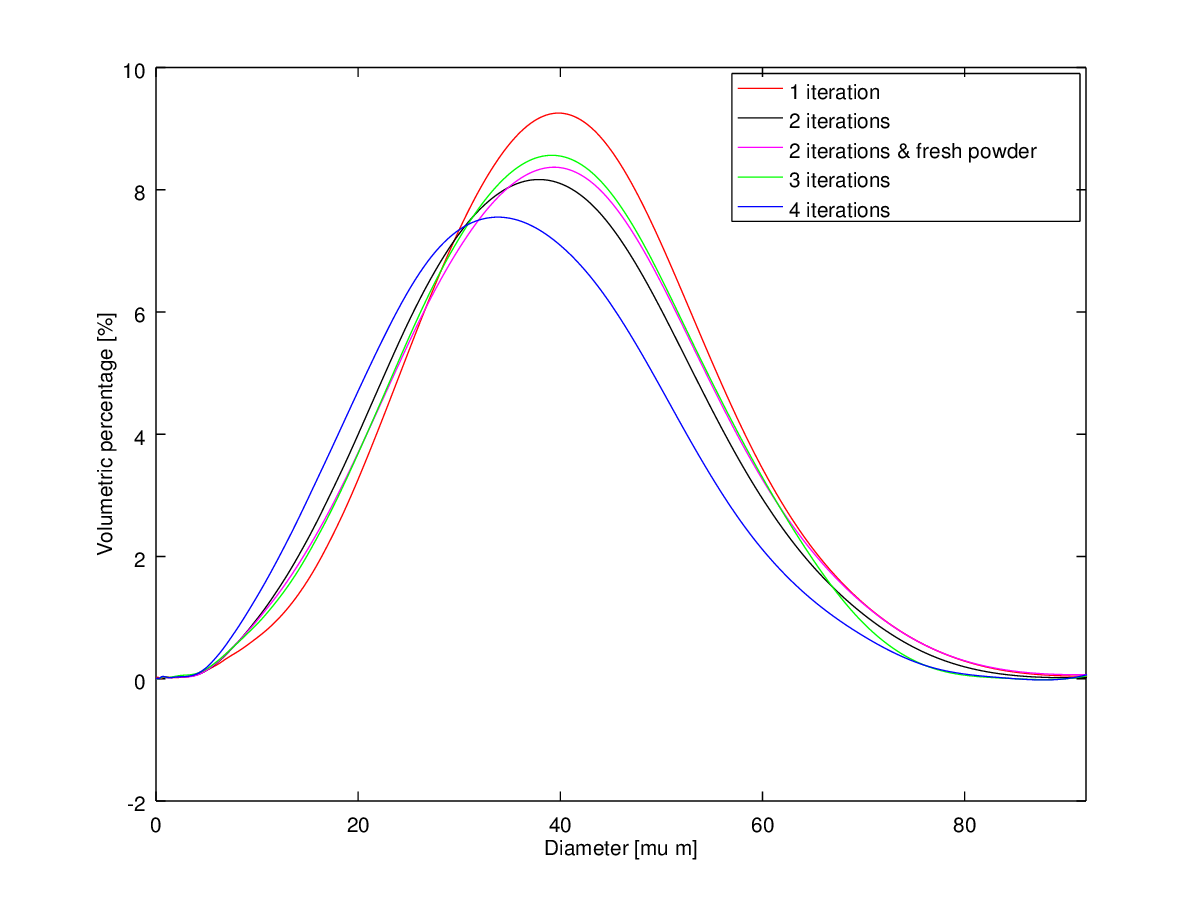
\includegraphics[scale=0.7]{Images/Granulo}
	\decoRule
	\caption[Powder size distributions for different batches.]{Powder size distributions for different batches.}
	\label{fig:granulo}
\end{figure}



\subsection{Composition}

\subsubsection{Fresh powder}

The composition of a sample of fresh powder was estimated through inductively coupled plasma (ICP) spectrometry. The result is shown in table \ref{tab:compoF}. Each mass fraction is vitiated by an error than can go up to 3[\%]. 
 \begin{center}
\begin{table}[ht]
\centering
\begin{tabular}{|c|c |c |c| }
    \hline
    %\multicolumn{4}{c}{Composition [\%wt]} \vline \\
\hline
    Al [\%wt]& Fe [\%wt]&Mg [\%wt]&Si [\%wt]\\
\hline 
\hline   
    89.0&0.14&0.50&9.99\\
    \hline
\end{tabular}

\caption[Composition of fresh AlSi10Mg powder]{Composition of fresh AlSi10Mg powder}
\label{tab:compoF}
\end{table}
 \end{center}


\subsubsection{Recycled powder}

\begin{figure}[ht]
\centering
\noindent\makebox[\textwidth]{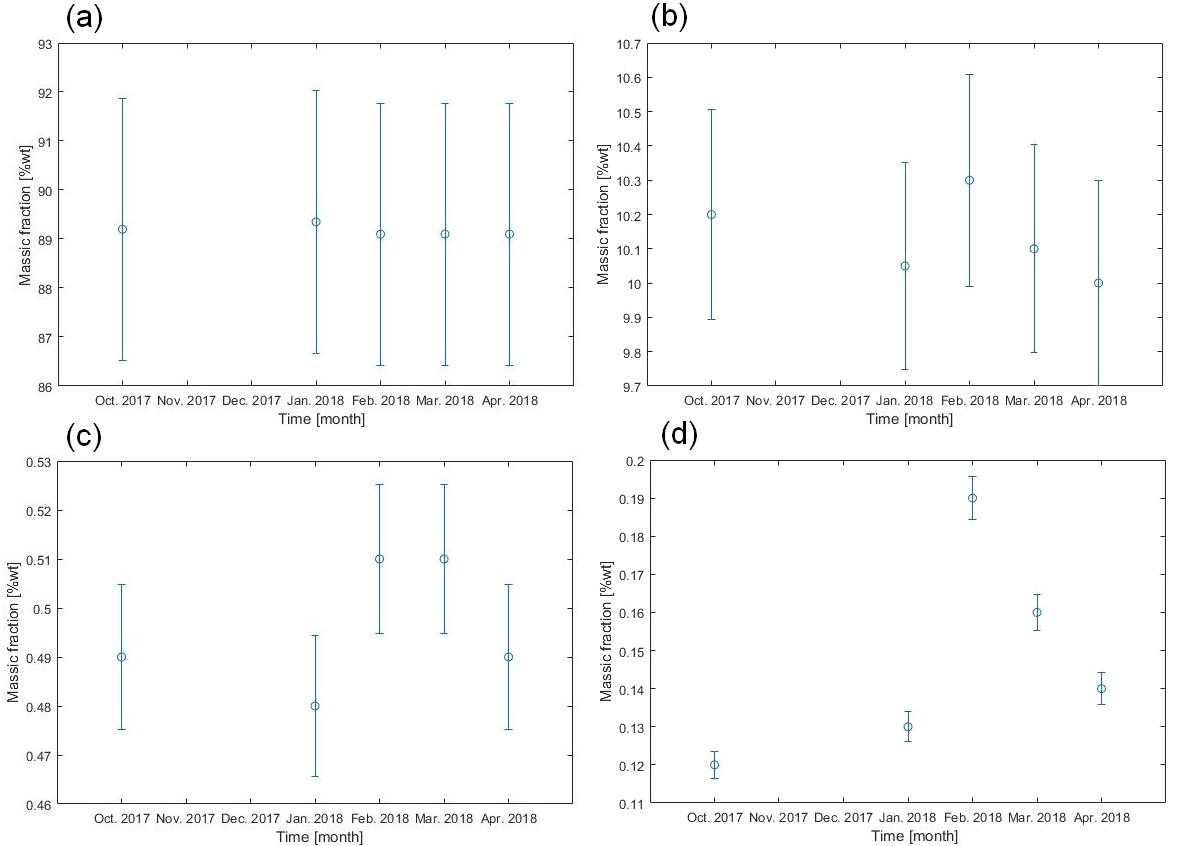
\includegraphics[scale=0.5]{Images/Compo}}
\decoRule
\caption[...(a) aluminium mass fraction (b) silicon mass fraction (c) magnesium mass fraction (d) iron mass fraction]{...(a) aluminium mass fraction (b) silicon mass fraction (c) magnesium mass fraction (d) iron mass fraction}
\label{fig:Compo}
\end{figure} 


 \begin{center}
\begin{table}[ht]
\noindent\makebox[\textwidth]{\begin{tabular}{|c|c |c |c| c|}
    \hline
    Date of sampling& \multicolumn{4}{c}{Composition [\%wt]} \vline\\
    \cline{2-5}
    & Al& Fe&Mg&Si\\
\hline 
\hline   
    23/10/2017  &89.2&0.12&0.49&10.2\\
    09/01/2018 & 89.3 & 0.13 &0.48&10.1\\
    12/01/2018 & 89.4 & 0.13 &0.48&10\\
    21/02/2018&89.1&0.19&0.51&10.3\\
    13/03/2018 &89.1&0.16&0.51&10.1\\    
    17/04/2018& 89.1 &0.14& 0.49 &10.0\\
    \hline
\end{tabular}}

\caption[Composition of recycled AlSi10Mg powder as a function of the date]{Composition of recycled AlSi10Mg powder as a function of the date}
\label{tab:compo}
\end{table}
 \end{center}

\section{Density and hardness study}
\subsection{Optimisation of the SLM parameters}
\label{Rparaopti}
The optimisation of the manufactured samples properties was done with respect to $\rho_{a,rel}$ and $H_v$. For this purpose, twelve cubes were fabricated with P varying from 0.75\% $P_{max} $to $P_{max}$ and $v_s$ from 900 to 1500 [$\frac{mm}{sec}$]. Details about batch X200-171024 are given in appendix \ref{AppendixA}. The goal of this optimisation was to select a single set of parameters values to use in the rest of the thesis. The parameters values were chosen to cover a wide range of $E_d$. Sets of parameters ($P=75\% P_{max}$ ; $v_s=1200 [\frac{mm}{sec}]$) and ($P=75\% P_{max}$ ; $v_s=900 [\frac{mm}{sec}]$) gave the best results in terms of $\rho_{a,rel}$ in a previous study done at UCL. It was decided to produce samples with these sets of values in triplicate in order to have a first insight on the process reproducibility. This will be discussed further in next section. Here, only the mean $H_v$ and $\rho_{a,rel}$ of those samples will be compared to the others'.\\

Results for the measurements of $\rho_{a,rel}$ and $H_v$ are summarised in figure \ref{fig:HD2-171024} and detailed in appendix \ref{AppendixA}. The 95\% confidence intervals (CI) are drawn on the graphs. The methods used to compute them are described in appendix \ref{AppendixC}. All apparent relative density values were obtained through hydrostatic weighing of the unpolished AB specimens.\\

\begin{figure}[ht]
\centering
\noindent\makebox[\textwidth]{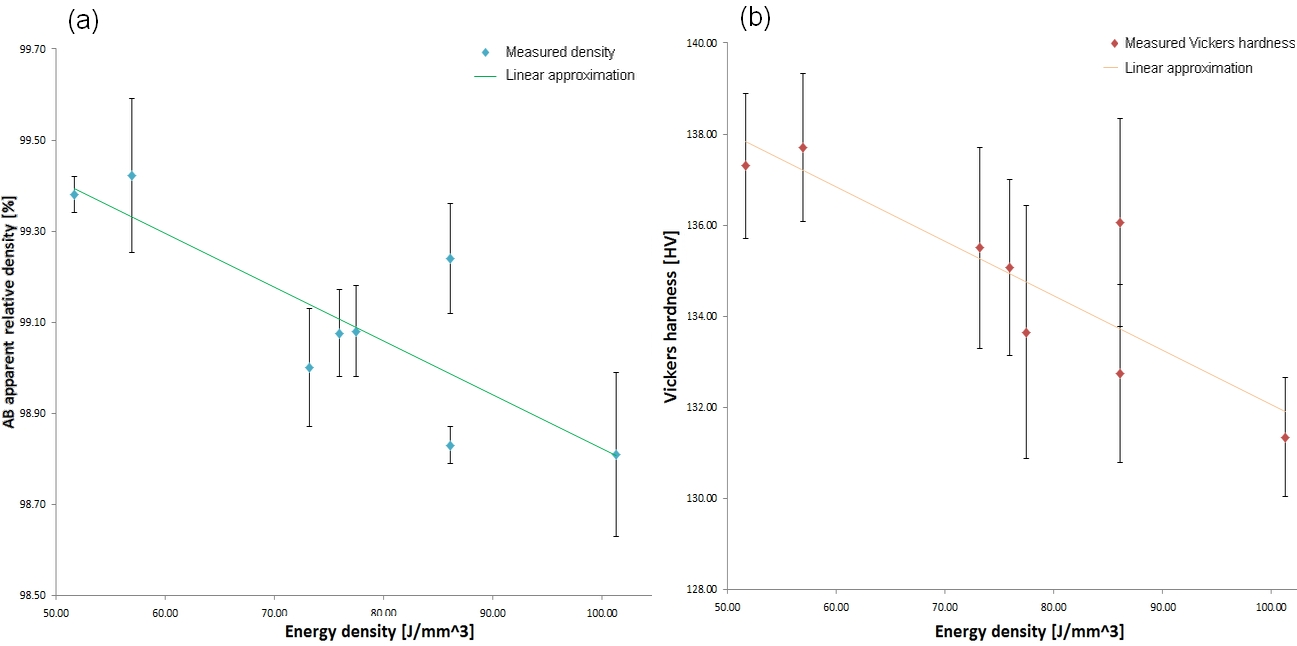
\includegraphics[scale=0.5]{Images/HD2-171024}}
\decoRule
\caption[Batch X200-171024 samples properties as a function of the energy density: (a) as-built apparent relative density (b) Vickers hardness]{Batch X200-171024 samples properties as a function of the energy density: (a) as-built apparent relative density (b) Vickers hardness}
\label{fig:HD2-171024}
\end{figure} 

 The graph shows a general progressive decrease of  $\rho_{a,rel}$ and $H_v$ for $E_d>57 [\frac{J}{mm^3}]$. The lower density and hardness measures at $E_d \simeq 86.12$ correspond to the parameters values ($P=P_{max}$ ; $v_s=1059 [\frac{mm}{sec}]$).


\subsection{Reproducibility}
\label{RReprod}
%\subsubsection{Relative density and hardness}
\subsubsection{General results}
Batch X200-171024 uncovered a reproducibility issue. One sample of type ($P=75\% P_{max}$ ; $v_s=900 [\frac{mm}{sec}]$) had a relative density $\simeq 5 [\%]$ lower than the others' ($\rho_{a,rel}=98.77[\%]$). It was decided to produce a batch of fifteen ($P=75\% P_{max}$ ; $v_s=1200 [\frac{mm}{sec}]$) cubic samples and fifteen ($P=75\% P_{max}$ ; $v_s=900 [\frac{mm}{sec}]$) others in order to assess the process reproducibility when using a same powder. The two sets of parameters were used to compare the results for optimal and sub-optimal set values. A total of 18 samples were fabricated close to one another (see \ref{fig:180109-real}) to see if the specimens rapprochement has any effect on their final properties. The distance between two adjacent cubes flanks in the same row (that is quasi-aligned with y) is $\simeq 50 [mm]$. The distance separating the rows is $\simeq 70 [mm]$. The apparent relative density was once more measured with the unpolished AB samples.\\

 \begin{center}
\begin{table}[ht]
\noindent\makebox[\textwidth]{\begin{tabular}{|c|c|c |c |c|}
    \hline
    Type & $\overline{\rho_{a,rel}}$ [\%] & $SD_{\rho_{a,rel}}$[\%]& $\overline{H_v}$ [HV]& $SD_{H_v}$[HV]\\

\hline
\hline   
    ($P=75\% P_{max}$ ; $v_s=1200 [\frac{mm}{sec}]$) & 99.42 & 0.08 & 138 & 0.4 \\
    ($P=75\% P_{max}$ ; $v_s=900 [\frac{mm}{sec}]$) & 99.08 & 0.27 & 135 & 1.3 \\
\hline

\end{tabular}}

\caption[Standard deviations and average values for apparent relative densities and hardnesses of the specimens of batch X200-171024]{Standard deviations and average values for apparent relative densities and hardnesses of the specimens of batch X200-171024}
\label{tab:78}
\end{table}
 \end{center}

Hardness and apparent relative density results for batch X200-180109 are shown in appendix \ref{AppendixA}. The key information is displayed in tables \ref{tab:78b} and \ref{tab:78bb}. Type ($P=75\% P_{max}$ ; $v_s=900 [\frac{mm}{sec}]$) samples exhibited slightly poorer properties than type ($P=75\% P_{max}$ ; $v_s=1200 [\frac{mm}{sec}]$) ones in average. However, the former have far better properties to what one could have expected based on previous results (see table \ref{tab:78}). The highest measured density is 99.54 [\%].\\

%\begin{figure}[ht]
%\centering
%\centerline{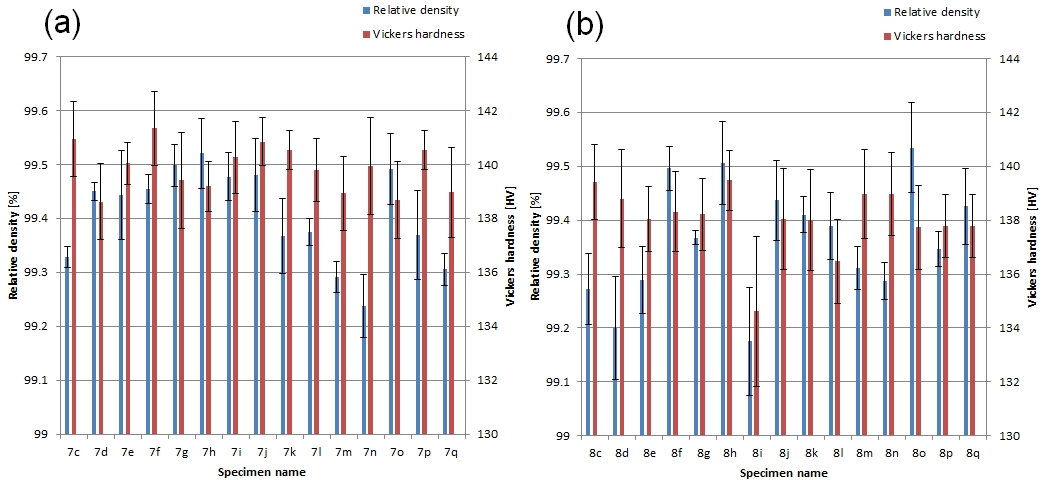
\includegraphics[scale=0.65]{Images/HD-180109-both}}
%\decoRule
%\caption[As-built apparent relative density and hardness results of batch X200-180109 for (a) type ($P=75\% P_{max}$ ; $v_s=1200 [\frac{mm}{sec}]$) samples (b) type ($P=75\% P_{max}$ ; $v_s=900 [\frac{mm}{sec}]$) samples.]{As-built apparent relative density and hardness results of batch X200-180109 for (a) type ($P=75\% P_{max}$ ; $v_s=1200 [\frac{mm}{sec}]$) samples (b) type ($P=75\% P_{max}$ ; $v_s=1200 [\frac{mm}{sec}]$) samples.}
%\label{fig:HD-171024}
%\end{figure} 



 \begin{center}
\begin{table}[ht]
\noindent\makebox[\textwidth]{\begin{tabular}{|c|c|c |c |c|}
    \hline
    Type & $\overline{\rho_{a,rel}}$ [\%] & $SD_{\rho_{a,rel}}$[\%]& $\overline{H_v}$ [HV]& $SD_{H_v}$[HV]\\

\hline
\hline   
    ($P=75\% P_{max}$ ; $v_s=1200 [\frac{mm}{sec}]$) & 99.40 & 0.09 & 139.9 & 0.87 \\
    ($P=75\% P_{max}$ ; $v_s=900 [\frac{mm}{sec}]$) & 99.36 & 0.11 & 138.3 & 1.3 \\


\hline
\end{tabular}}

\caption[Standard deviations and average values for apparent relative densities and hardnesses of the specimens of batch X200-180109]{Standard deviations and average values for apparent relative densities and hardnesses of types the specimens of batch X200-180109}
\label{tab:78b}
\end{table}
 \end{center}
 
 
 \begin{center}
\begin{table}[ht]
\noindent\makebox[\textwidth]{\begin{tabular}{|c|c|c |c |c|}
    \hline
    Type & $min(\rho_{a,rel})$ [\%] & $max(\rho_{a,rel})$[\%]& $ min(H_v)$ [HV]& $max(H_v)$[HV]\\

\hline
\hline   
    ($P=75\% P_{max}$ ; $v_s=1200 [\frac{mm}{sec}]$)  & 99.24 & 99.52 & 138.6 & 141.4 \\
    ($P=75\% P_{max}$ ; $v_s=900 [\frac{mm}{sec}]$) & 99.18 & 99.54 & 134.6 & 140.4 \\


\hline
\end{tabular}}

\caption[Minimal and maximal values for apparent relative densities and hardnesses of the specimens of batch X200-180109]{Minimal and maximal values for apparent relative densities and hardnesses of the specimens of batch X200-180109}
\label{tab:78bb}
\end{table}
 \end{center}

\subsubsection{Sample proximity and position influence}
The results are displayed in figure \ref{fig:180109-HD} as functions of the (x,y) positions of the samples on the manufacturing plate. The coordinated are such that the roll sweeps were done in the positive $x$ direction during the fabrication. Other graphs showing the averaged $\rho_{a,rel}$ and $H_v$ as functions of the x and y coordinates were also plotted. To do so, the samples distanced from less than 1 [cm] along x or y were considered to have the same corresponding coordinate. The graphs are shown in appendix \ref{AppendixD}. No significant trend was observed on these graphs: the variations of hardnesses and relative densities are too small compared to the CI. \\
\begin{figure}[h!]
\centering
\centerline{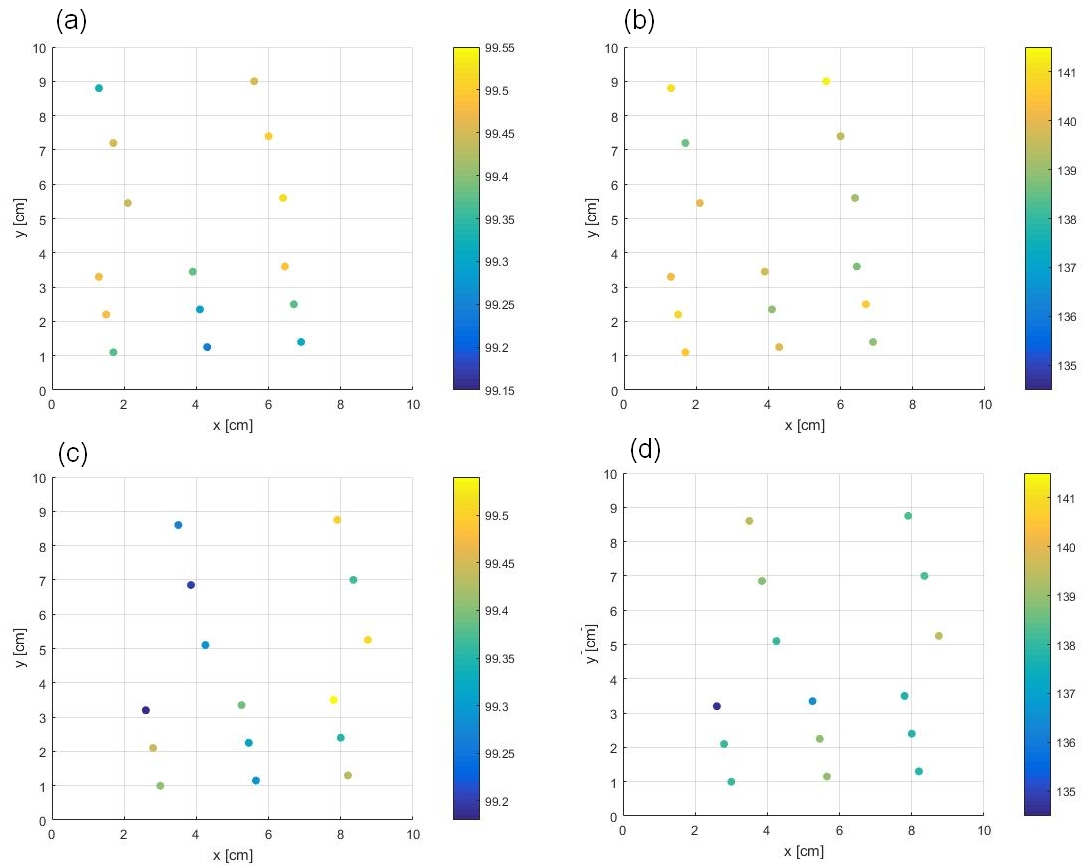
\includegraphics[scale=0.62]{Images/180109-HD}}
\decoRule
\caption[Batch X200-180109 scatter plots as functions of the (x,y) position on the manufacturing plate: (a) type (P=0.75 $Pmax$; $v_s$=1200 $\frac{mm}{sec}$) apparent relative densities (b) type (P=0.75 $Pmax$; $v_s$=1200 $\frac{mm}{sec}$) hardnesses (c) type (P=0.75 $Pmax$; $v_s$=900 $\frac{mm}{sec}$) apparent relative densities (d) type (P=0.75 $Pmax$; $v_s$=900 $\frac{mm}{sec}$) hardnesses]{Batch X200-180109 scatter plots as functions of the (x,y) position on the manufacturing plate: (a) type (P=0.75 $Pmax$; $v_s$=1200 $\frac{mm}{sec}$) apparent relative densities (b) type (P=0.75 $Pmax$; $v_s$=1200 $\frac{mm}{sec}$) hardnesses (c) type (P=0.75 $Pmax$; $v_s$=900 $\frac{mm}{sec}$) apparent relative densities (d) type (P=0.75 $Pmax$; $v_s$=900 $\frac{mm}{sec}$) hardnesses}
\label{fig:180109-HD}
\end{figure} 

A comparison of the results for closely packed samples (y<6) and distant ones (y>6) was also carried out. The details are shown in tables \ref{tab:CPD} and  \ref{tab:CPD2}. Again, no significant distinction could be drawn between the two.

 \begin{center}
\begin{table}[ht]
\noindent\makebox[\textwidth]{\begin{tabular}{|c|c|c|c |c |c|}
    \hline
    Type & Position& $\overline{\rho_{a,rel}}$ [\%] & $SD_{\rho_{a,rel}}$[\%]& $\overline{H_v}$ [HV]& $SD_{H_v}$[HV]\\

\hline
\hline   
    ($P=75\% P_{max}$ ; $v_s=1200 [\frac{mm}{sec}]$) & y>6& 99.45 & 0.07 & 140.0 & 1.1 \\
         & y<6& 99.38 & 0.07 & 139.9 & 0.7 \\
    ($P=75\% P_{max}$ ; $v_s=900 [\frac{mm}{sec}]$) & y>6& 99.36 & 0.10 & 138.7 & 0.6 \\
    & y<6& 99.37 & 0.08 & 138.0 & 1.6 \\


\hline
\end{tabular}}

\caption[Standard deviations and average values for apparent relative densities and hardnesses of the specimens of batch X200-180109]{Standard deviations and average values for apparent relative densities and hardnesses of types the specimens of batch X200-180109}
\label{tab:CPD}
\end{table}
 \end{center}
 
 
 \begin{center}
\begin{table}[ht]
\noindent\makebox[\textwidth]{\begin{tabular}{|c|c|c |c |c|c|}
    \hline
    Type & Position & $min(\rho_{a,rel})$ [\%] & $max(\rho_{a,rel})$[\%]& $ min(H_v)$ [HV]& $max(H_v)$[HV]\\

\hline
\hline   
    ($P=75\% P_{max}$ ; $v_s=1200 [\frac{mm}{sec}]$)&y>6 & 99.33 & 99.52 & 138.6 & 141.4 \\
    &y<6 & 99.24 & 99.49 & 138.7 & 140.9 \\
    ($P=75\% P_{max}$ ; $v_s=900 [\frac{mm}{sec}]$) &y>6& 99.20 & 99.51 & 138.0 & 139.5 \\
    &y<6& 99.29 & 99.54 & 134.6 & 140.4 \\


\hline
\end{tabular}}

\caption[Minimal and maximal values for apparent relative densities and hardnesses of the specimens of batch X200-180109]{Minimal and maximal values for apparent relative densities and hardnesses of the specimens of batch X200-180109}
\label{tab:CPD2}
\end{table}
 \end{center}


\subsubsection{Scan order influence}
The apparent relative densities, Vickers hardnesses and the corresponding 95 \% CI are displayed as functions of the scan order in figure \ref{fig:180109-SO}. The period of time between two successive scans of powder layers is the same for every sample. However, the time span between the scan and the powder covering differs from one to the other. This could lead to differences in terms of thermal exchanges.\\

\begin{figure}[ht]
\centering
\centerline{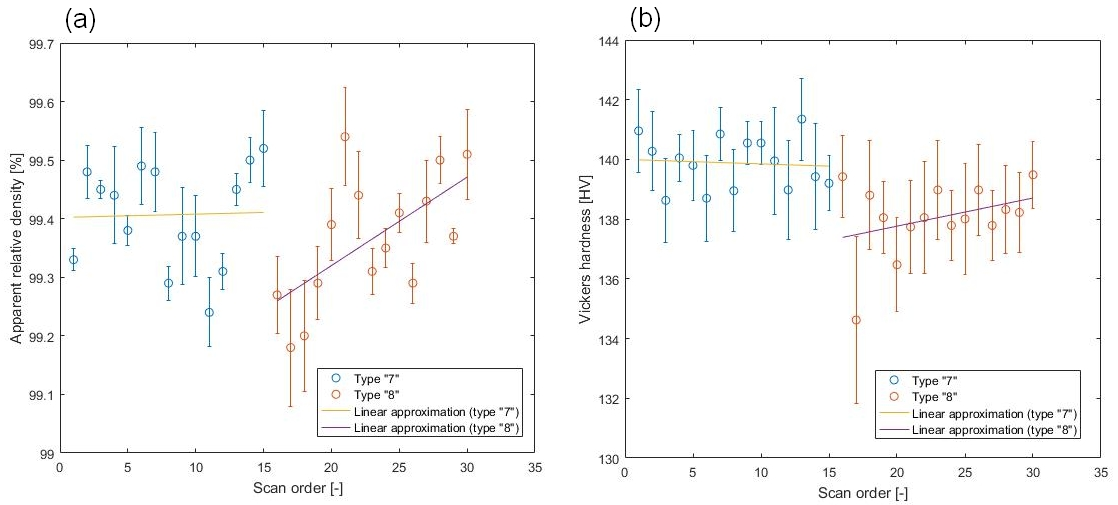
\includegraphics[scale=0.62]{Images/180109-SO}}
\decoRule
\caption[Batch X200-180109 scatter plots as functions of the scan order of (a) the apparent relative densities (b) the Vickers hardnesses]{Batch X200-180109 scatter plots as functions of the scan order of (a) the apparent relative densities (b) the Vickers hardnesses}
\label{fig:180109-SO}
\end{figure} 

Only one trend can be noted: the density of the ($P=75\% P_{max}$ ; $v_s=900 [\frac{mm}{sec}]$) samples appears to be larger for later scanning. However, this doesn't help understanding the poorer properties measured for samples with the same parameters in batch X200-171024 as they were precisely the last scanned. \\

\subsubsection{Powder influence}

The hardnesses and relative densities of samples manufactured using the optimised parameters ($P=75\% P_{max}$ ; $v_s=1200 [\frac{mm}{sec}]$) were monitored throughout this whole work. In this way, it was possible to study the impact of the powder ageing. Control cubes of dimensions 10x10x10 [$mm^3$] were produced in multiple batches for that purpose. The average measurements for those samples are gathered in table \ref{tab:control}. Detailed information is given in appendix \ref{AppendixA}.\\

 \begin{center}
\begin{savenotes}
 \begin{table}[ht]
\noindent\makebox[\textwidth]{\begin{tabular}{|c|c|c |c |c|}
    \hline
    Batch & $\overline{\rho_{a,rel}}$ \footnote{Measured by HW (AB)} [\%]  & $\overline{\rho_{a,rel}}$ \footnote{Measured by HW (polished)} [\%]  & $\overline{\rho_{rel}}$ \footnote{Measured by RODIA} [\%]  & $\overline{H_v}$ [HV]\\

\hline
\hline   
    X200-171024&99.42 & - & - & 137.7 \\
    X200-170109&99.40 & 99.51  & 99.59 & 139.9 \\
    X200-170319&- &  99.75  & 99.84 & 139.8 \\
    X200-170417&- &  99.47  & 99.67 & 136.0 \\
\hline
\end{tabular}}

\caption[Average hardness and relative density measurements for the control cubes of each batch]{Average hardness and relative density measurements for the control cubes of each batch}
\label{tab:control}
\end{table}
\end{savenotes}
 \end{center}

Samples from batches X200-180222 and X200-180228 are not included in this section. In those cases, fresh steamed powder was used, which induced high porosity in the produced parts. The most reasonable explanation is that the powder processing caused the formation of aggregates. This was not investigated further, and only recycled powder was employed thereafter. Table \ref{taqb:control} indicates that the relative density peaked with batch X200-170419. It dropped slightly afterwards with batch X200-170417. Hardness also decreased - more significantly - with this last batch.\\


\subsection{Homogeneity}
As said in section \ref{MMFPP}, all tensile specimens were fabricated vertically. Their height is significantly greater than the other samples'; respectively 6 [cm], and 1 [cm] or less. It was chosen to cut up specimen X200-180417-25 into slices to measure if the density and hardness were homogeneous along the Z direction in the material. The surfaces analysed were named according to their original Z position in the specimen with "B", "C1" , "C2", "C3" and "T" (for bottom, center and top) and to the test done with a letter "D" or "H"  (for density and hardness). The denomination is summarised in figure \ref{fig:saus}.\\

\begin{figure}[ht]
\centering
\centerline{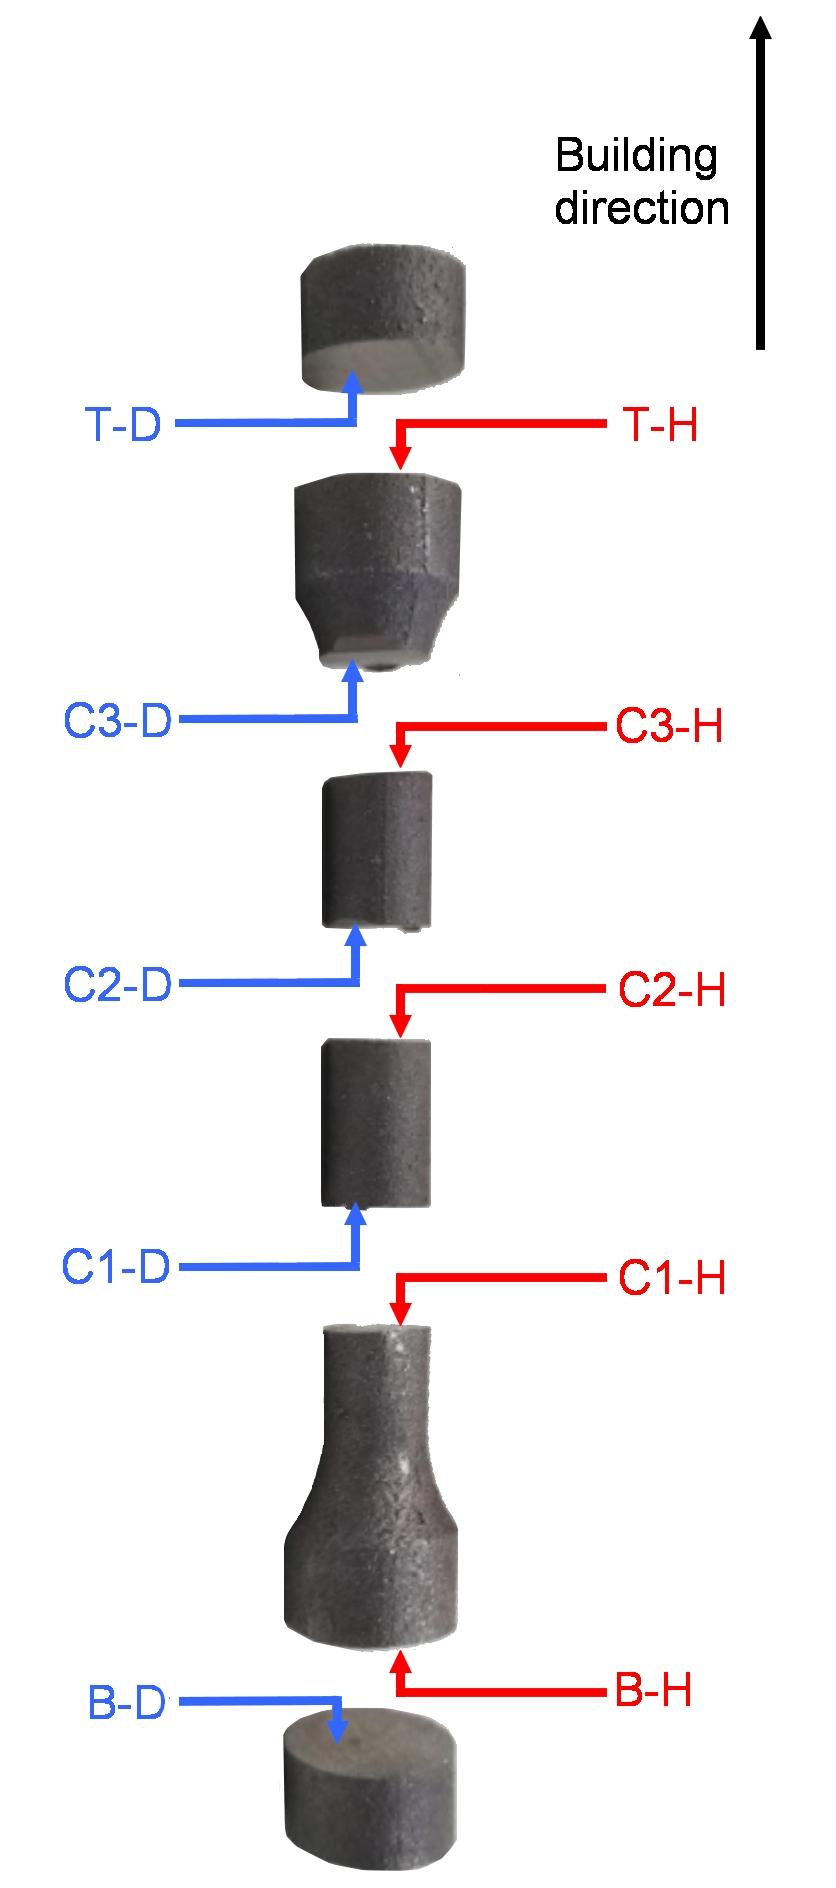
\includegraphics[scale=0.23]{Images/Saus}}
\decoRule
\caption[Specimen X200-180417-25 sub-parts and surfaces denomination]{Specimen X200-180417-25 sub-parts and surfaces denomination.}
\label{fig:saus}
\end{figure}

Results are shown in figure \ref{fig:HD-180417}. With regard to hardness, no general trend could be observed. The measured values are high and closely packed except for the "B" surface, which exhibited a significantly lower hardness. Density values are all equal or above 99.75 [\%]. The values at the center of the sample were slightly lower to the extremities'. A summary of the results is displayed in table \ref{tab:25}.

 \begin{center}
	\begin{table}[ht]
		\begin{tabular}{|c|c |c |c| c|}
			\hline
			Property& Average value & Minimum & Maximum & Standard deviation \\
			\hline 
			\hline   
			Relative density [\%] & 99.80 & 99.75 & 99.87 & 0.05\\
			Hardness [HV] &138.0 &132.2 &141.7&3.5\\
			\hline
		\end{tabular}

		\caption[Relative density and hardness results summary for specimen X200-180417-25 surfaces]{Relative density and hardness results summary for specimen X200-180417-25 surfaces}
		\label{tab:25}
	\end{table}
\end{center}


\begin{figure}[ht]
\centering
\centerline{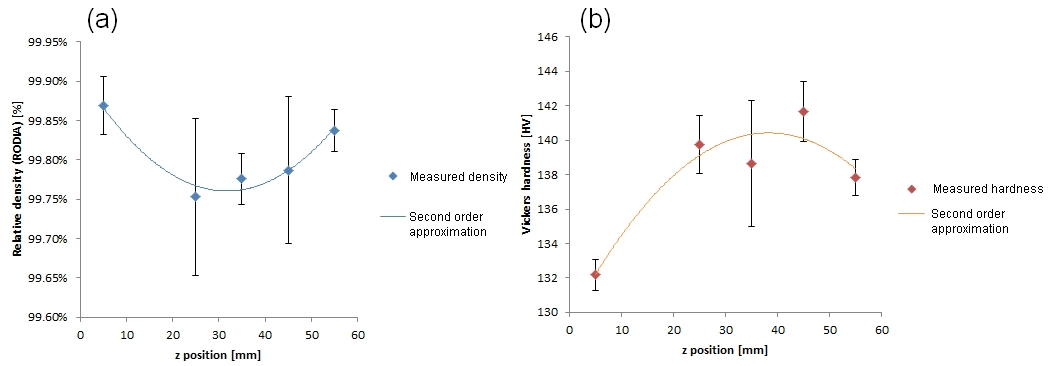
\includegraphics[scale=0.62]{Images/SausHD}}
\decoRule
\caption[Scatter plots of the results for specimen X200-180417-25 surfaces as a function of the vertical position: (a) RODIA based relative density (b) Vickers hardness]{Scatter plots of the results for specimen X200-180417-25 surfaces as a function of the vertical position: (a) RODIA based relative density (b) Vickers hardness}
\label{fig:HD-180417}
\end{figure} 


\section{Characterisation of the as-built samples} 
\label{RCABS}
\subsection{Melt pools sizes and distribution}

Samples "8a" and "8b" of batch X200-171024 were fabricated using the same manufacturing parameters. However, the former had way lower $\rho_{a,rel}$ and $H_v$ (see appendix \ref{AppendixA}). A statistical analysis of the melt pools size distribution was conducted for both samples to try grasping a better understanding of the origin of the differences. The procedure described in section \ref{MMOM} was followed. 130 zones were manually delineated for both samples. An illustration of the zones subdivision is shown on figure \ref{fig:B1}.\\

\begin{figure}[ht]
\centering
\centerline{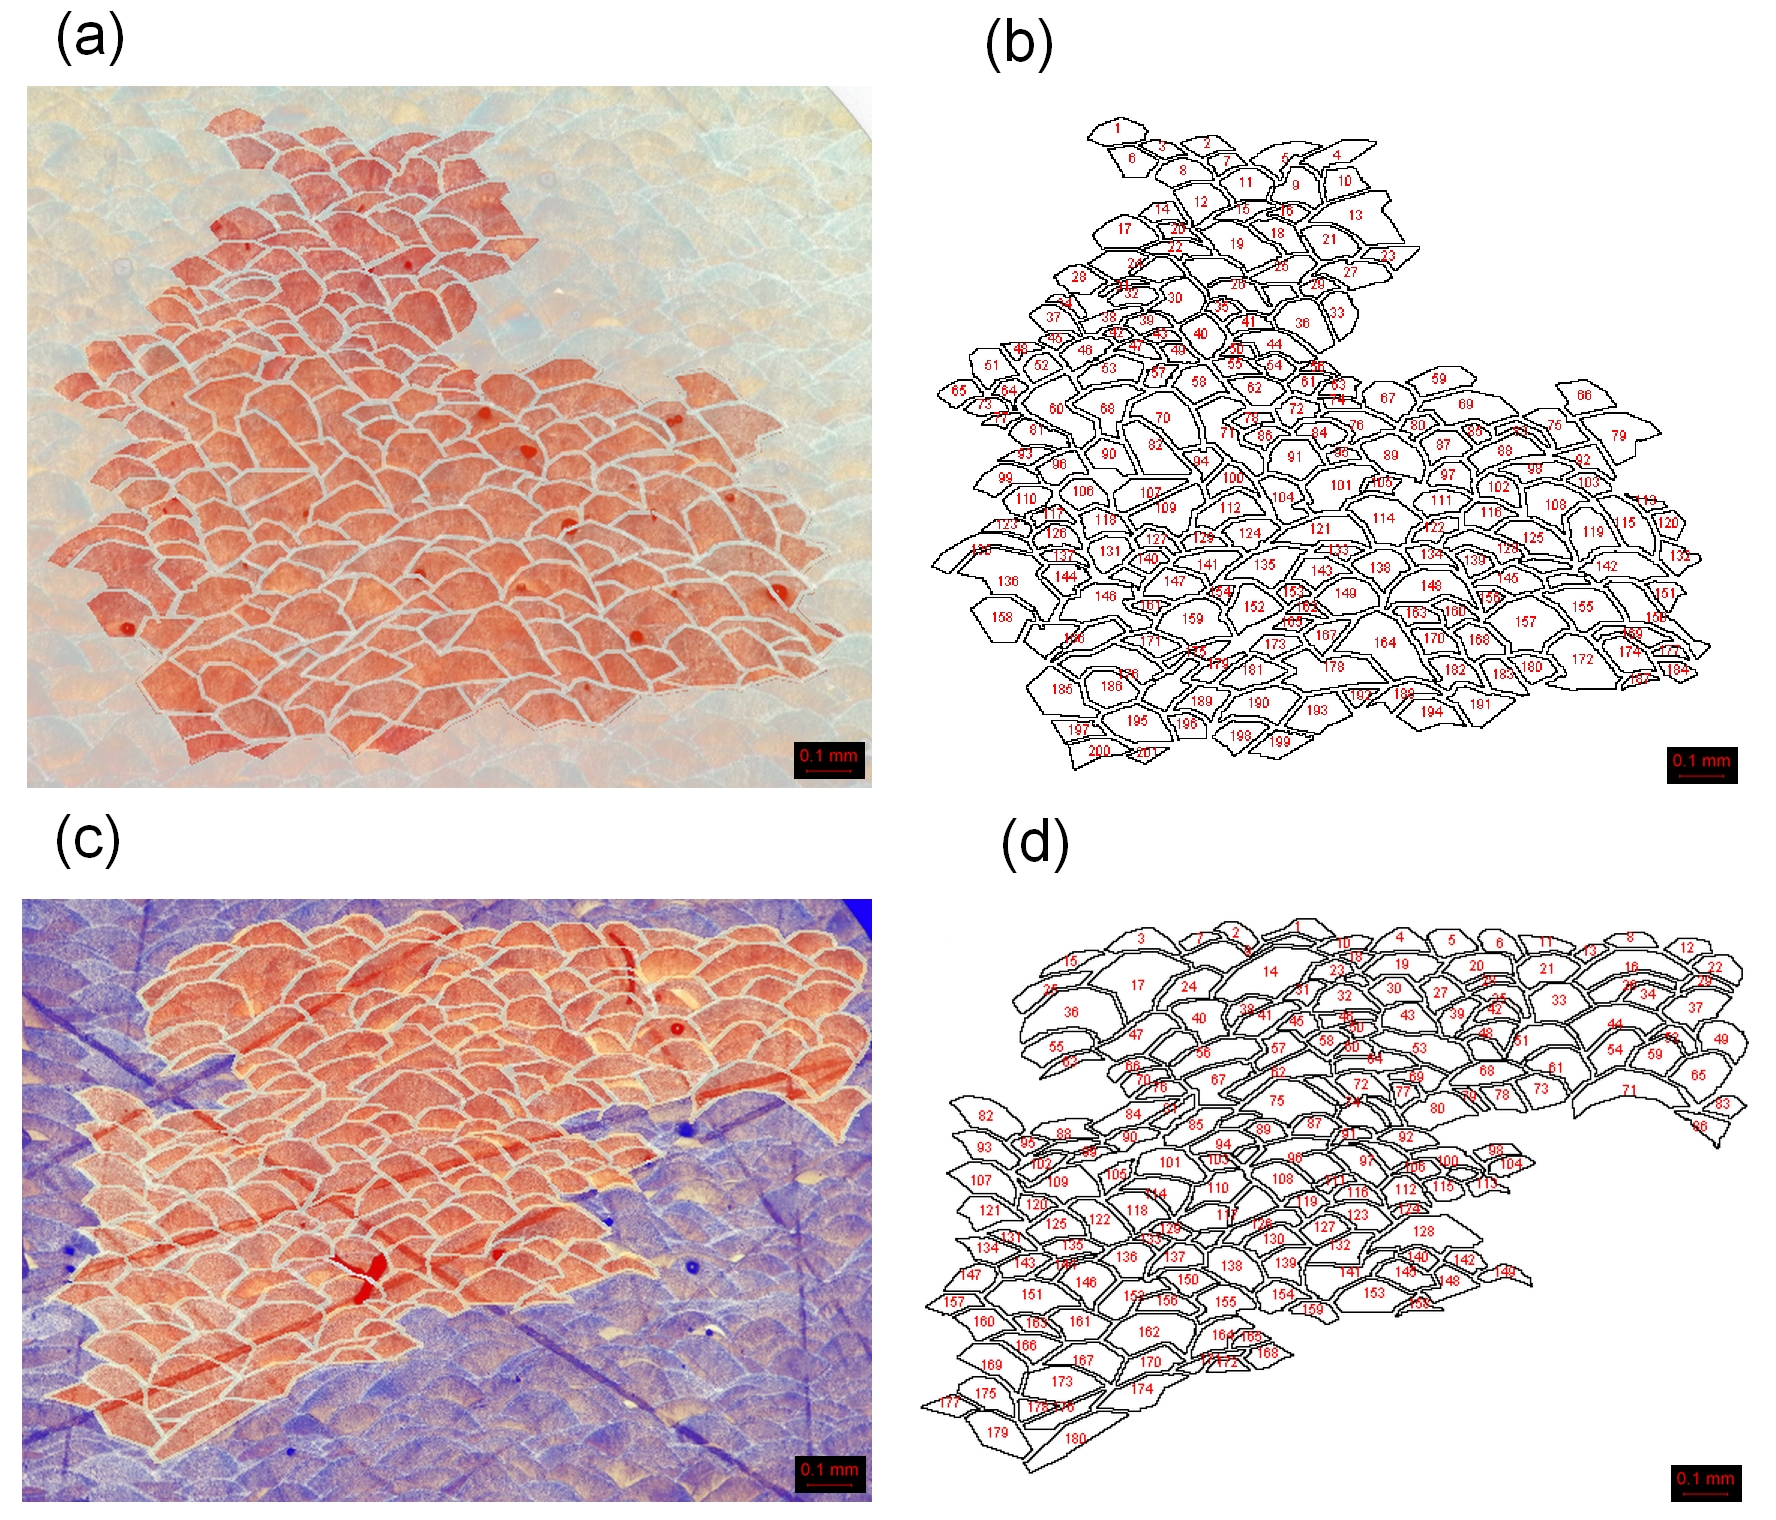
\includegraphics[scale=0.12]{Images/B1}}
\decoRule
\caption[Screen captures of (a) melt pools subdivision from a picture of specimen "8a" (b) \textit{ImageJ} partitioning from the same picture of specimen "8a" (c) melt pools subdivision from a picture of specimen "8b" (d) \textit{ImageJ} partitioning from the same picture of specimen "8b"]{Screen captures of (a) melt pools subdivision from a picture of specimen "8a" (b) \textit{ImageJ} partitioning from the same picture of specimen "8a" (c) melt pools subdivision from a picture of specimen "8b" (d) \textit{ImageJ} partitioning from the same picture of specimen "8b"}
\label{fig:B1}
\end{figure} 

In both cases, the area of every zone was computed. Melt pools areas histograms are displayed on figure \ref{fig:HistB1}. Even though the mean areas are nearly the same, the distributions are quite different (see table ). The standard deviation for sample "8b" is approximately 50[\%] bigger than for "8a" one. The corresponding picture contains significantly more melt pools with small areas (<200 [$\mu m^2$]) and large ones (>1000 [$\mu m^2$]). \\

\begin{figure}[ht]
\centering
\centerline{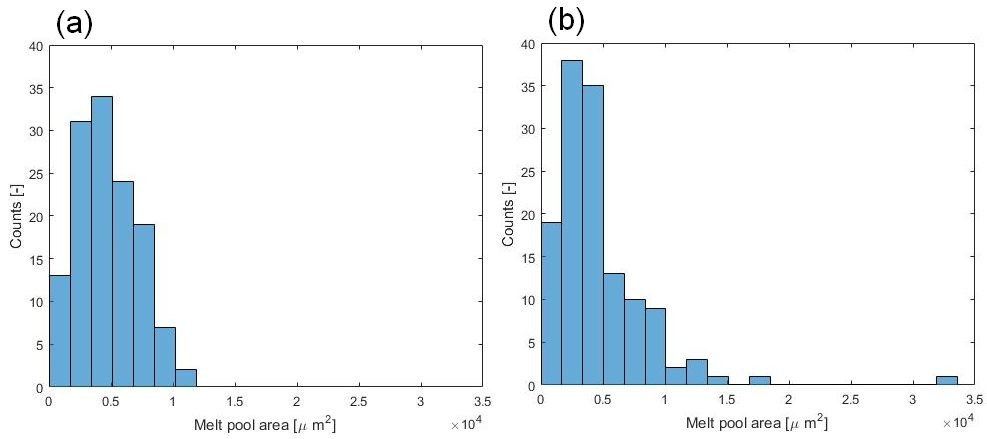
\includegraphics[scale=0.7]{Images/HistB1}}
\decoRule
\caption[Histograms of melt pools areas occurrences from \textit{ImageJ} partitioning of (a) sample "8a"  b) sample "8b"]{Histograms of melt pools areas occurrences from \textit{ImageJ} partitioning of (a) sample "8a"  b) sample "8b"}
\label{fig:HistB1}
\end{figure} 

 \begin{center}
\begin{table}[ht]
\noindent\makebox[\textwidth]{\begin{tabular}{|c |c |c|}
    \hline
     Sample & Mean area [$\mu m^2$] & SD [$\mu m^2$] \\

\hline
\hline   
    "8a" & 4.6629 $10^3$ & 2.3625 $10^3$  \\
    "8b" & 4.6597 $10^3$ & 3.9285 $10^3$  \\
    \hline
\end{tabular}}

\caption[Summary of the melt pools areas distributions for samples "8a" and "8b"]{Summary of the melt pools areas distributions for samples "8a" and "8b"}
\label{tab:tracMAB}
\end{table}
 \end{center}

\subsection{Microstructure}
Optique: Porosité en grande majorité aux interfaces des bains de fusion. Grandes zones non fondues (?).

\subsection{Residual stresses}

\subsection{Mechanical properties}

The average tensile properties of the six tested as-built specimens are displayed in table \ref{tab:tracMAB}. Detailed information may be consulted in appendice \ref{AppendixAbis}. All data was computed based on the procedures of section \ref{MMTT}.\\

 \begin{center}
\begin{table}[ht]
\noindent\makebox[\textwidth]{\begin{tabular}{|c |c |c| c|}
    \hline
     E [GPa] & $\sigma_y$ [MPa] & $\sigma_u$ [MPa] & $\epsilon_f$[\%] \\

\hline
\hline   
    64.9 $\pm 3.0$ & 266.6 $\pm 23.6$ & 381.7 $\pm 24.7$ & 2.5 $\pm 0.5$  \\

    \hline
\end{tabular}}

\caption[Average tensile mechanical properties of the as-built specimens from batch X200-180417]{Average tensile mechanical properties of the as-built specimens from batch X200-180417}
\label{tab:tracMAB}
\end{table}
 \end{center}
 
One specimen built with no contour scanning strategy was tested. Its tensile behaviour was observed to be very similar to the other samples. No distinction shall thus be made between the two types in what follows. Stress-strain curve for specimen X200-180417-1 was non-linear before the plasticity regime started. This is due to slippage in the grips. The obtained Young's modulus for the test was thus not taken into account for the computation of the average value.\\

No necking phenomena was observed among all tensile tests for AB samples. The Considere criterion was used for the detection of plastic instability. It states that necking starts at $\frac{d\sigma_{true}}{d\epsilon_{true}}=\sigma$, which is equivalent to $\frac{d\sigma_{eng}}{d\epsilon_{eng}}=0$. This condition was not satisfied for any AB engineering stress-strain curve.\\
 
\section{Characterisation of the heat-treated samples}
\label{RCHTS}
\subsection{Microstructure}

\subsection{Residual stresses}

\subsection{Mechanical properties}

Tensile tests were made with heat treated specimens. All samples had undergone a HT during 2h, at either 150$^\circ C$, 200$^\circ C$, 250 $^\circ C$ or 300 $^\circ C$. Three samples were tested for each HT except for the one at 250 $^\circ C$ (only two samples). One specimen heated at 150$^\circ C$ was fabricated with no contour scanning strategy. The results are gathered in \ref{AppendixB}. The average tensile properties for each HT are shown in table \ref{tab:tracMHT}. All samples heated at 250$^\circ C$ and 300$^\circ C$ were observed to go through necking in the sense of Considère criterion. Their $\epsilon_f,true$ was computed thanks to a profile projector. \\

 \begin{center}
\begin{table}[ht]
\noindent\makebox[\textwidth]{\begin{tabular}{|c|c |c |c| c|c|}
    \hline
     HT & E [GPa] & $\sigma_y$ [MPa] & $\sigma_u$ [MPa] & $\epsilon_{f,eng}$[\%] & $\epsilon_{f,true}$ [\%] \\

\hline
\hline   
   150$^\circ$C (2h) & 68.4 $\pm 1.9$ & 288.2 $\pm 1.4$ & 441.7 $\pm 5.5$ & 5.5 $\pm 0.8$&-  \\
    200$^\circ$C (2h) &  72.1 $\pm 0.4$ & 245.4 $\pm 0.6$ & 382.0 $\pm 11.4$ & 4.6 $\pm 0.3$ &- \\
     250$^\circ$C (2h) &  70.6 $\pm 1.0$ & 235.1 $\pm 7.4$ & 340.9 $\pm 12.2$ &8.8 $\pm 0.2$ & 16.5 $\pm 0.1$  \\
      300$^\circ$C (2h) &  68.9 $\pm 0.6$ & 170.7 $\pm 1.7$ & 252.9 $\pm 10.4$ &13.6 $\pm 0.5$ & 29.7 $\pm 0.1$  \\

    \hline
\end{tabular}}

\caption[Average tensile mechanical properties of the heat-treated specimens from batch X200-180417]{Average tensile mechanical properties of the heat-treated specimens from batch X200-180417}
\label{tab:tracMHT}
\end{table}
 \end{center}

The heat treatment at 150$^\circ$ increased notably both $\sigma_u$ and $\epsilon_f$ compared to the as-built values. However, the heating at 200$^\circ$ caused virtually no change of ultimate tensile strength, and the fracture strain augmentation was weaker than the 150$^\circ C$ specimen's. For HT at 250$^\circ$ and 300$^\circ$, the material softened significantly (with necking appearance); the higher the heating temperature, the bigger the ductility increased and the strength decreased. The Young's modulus measured for heat treated samples was significantly bigger in average 69.9 [GPa] compared to 64.9 [GPa].\\

The average $\sigma_{true}$-$\epsilon_{true}$ data was also displayed in a graphical form for better insight. The true stress and strain were approximated by the engineering ones for samples with no necking. As the curves for a same HT do not end at the same $\epsilon_{f,true}$, the average curve could not be obtained by simply taking the mean $\sigma$ value at each $\epsilon$. This would have indeed lead to discontinuities at each fracture strain on the graph. The chosen solution was to fit the average properties in a Ramberg-Osgood hardening law:\\

$$\epsilon_{true}=\frac{\sigma_{true}}{E_a}+ 0.002(\frac{\sigma_{true}}{\sigma_{y,a}})^{(\frac{1}{n})}$$

where $n \simeq \epsilon_{f,true,a}$ is the strain hardening coefficient. The subscript "a" means that the average values are used. This was done with an online calculator \parencite{RO}. \\


\begin{figure}[ht]
\centering
\centerline{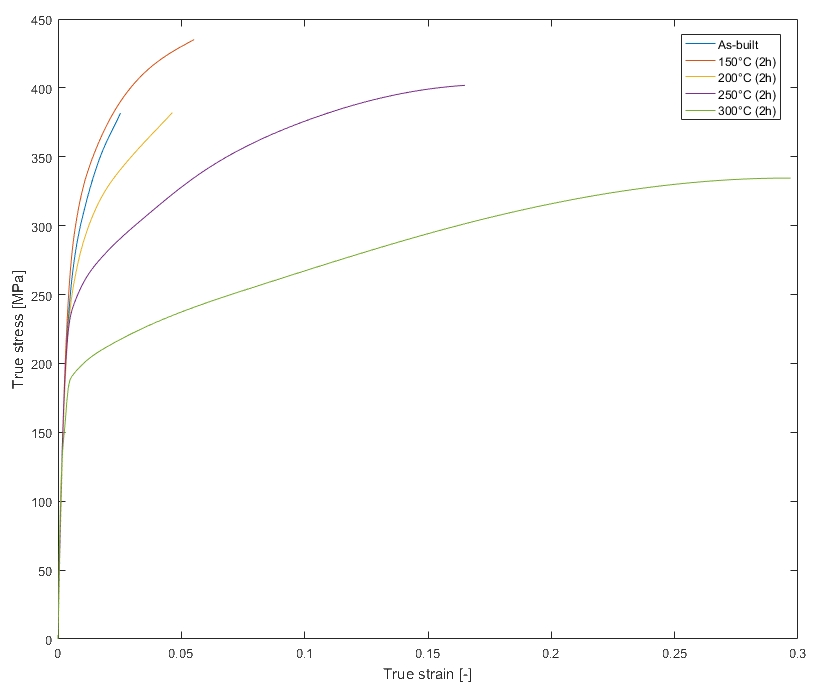
\includegraphics[scale=0.6]{Images/MeanTrac}}
\decoRule
\caption[Average stress-strain curves of the tensile specimens of batch X200-180417.]{Average stress-strain curves of the tensile specimens of batch X200-180417.}
\label{fig:MeanTrac}
\end{figure}

%\begin{table}
%\caption{The effects of treatments X and Y on the four groups studied.}
%\label{tab:treatments}
%\centering
%\begin{tabular}{l l l}
%\toprule
%\tabhead{Groups} & \tabhead{Treatment X} & \tabhead{Treatment Y} \\
%\midrule
%1 & 0.2 & 0.8\\
%2 & 0.17 & 0.7\\
%3 & 0.24 & 0.75\\
%4 & 0.68 & 0.3\\
%\bottomrule\\
%\end{tabular}
%\end{table}